\documentclass[12pt]{article}
\usepackage{enumerate}
\usepackage{notes}
\usepackage{oxford}

\begin{document}
\title{Oxford A1 - Differential Equations \footnotetext{\url{https://courses.maths.ox.ac.uk/node/5372}}}
\author{Dan Davison}
\maketitle

\section{Sheet 1}

\subsection*{}
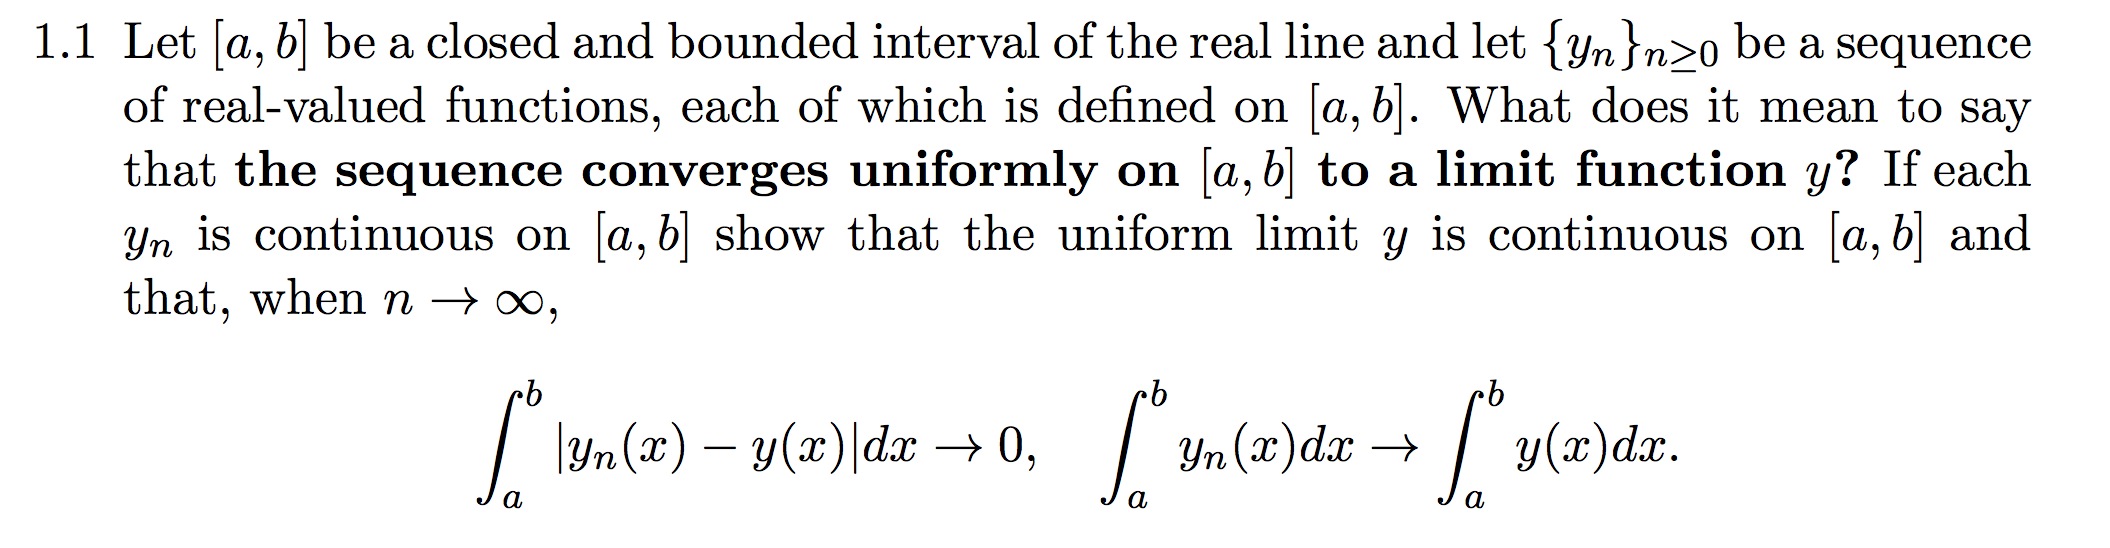
\includegraphics[width=450pt]{img/differential-equations-a1-1-1-a.png}\\
\begin{mdframed}
  \subsubsection*{(a) Definition of uniform convergence}
  The sequence of functions $\{y_n\}_{n\geq 0}$ \textbf{converges uniformly on
    $[a, b]$ to $y$} if and only if for all $\epsilon > 0$ there exists an
  $m \in \N$ such that for all $n > m$ and for all $x \in [a,b]$,
  $|y_n(x) - y(x)| < \epsilon$.

  \subsubsection*{(b) Show that the limit function is continuous}

  The claim is that if each $y_n$ is continuous on $[a,b]$ then $y$ is
  continuous on $[a,b]$. We are told that
  \begin{enumerate}
  \item $\{y_n\}_{n \geq 0}$ converges uniformly to $y$, and
  \item each $y_n$ is continuous on $[a,b]$.
  \end{enumerate}
  ~\\
  \textbf{Informal illustration of proof:}\\
  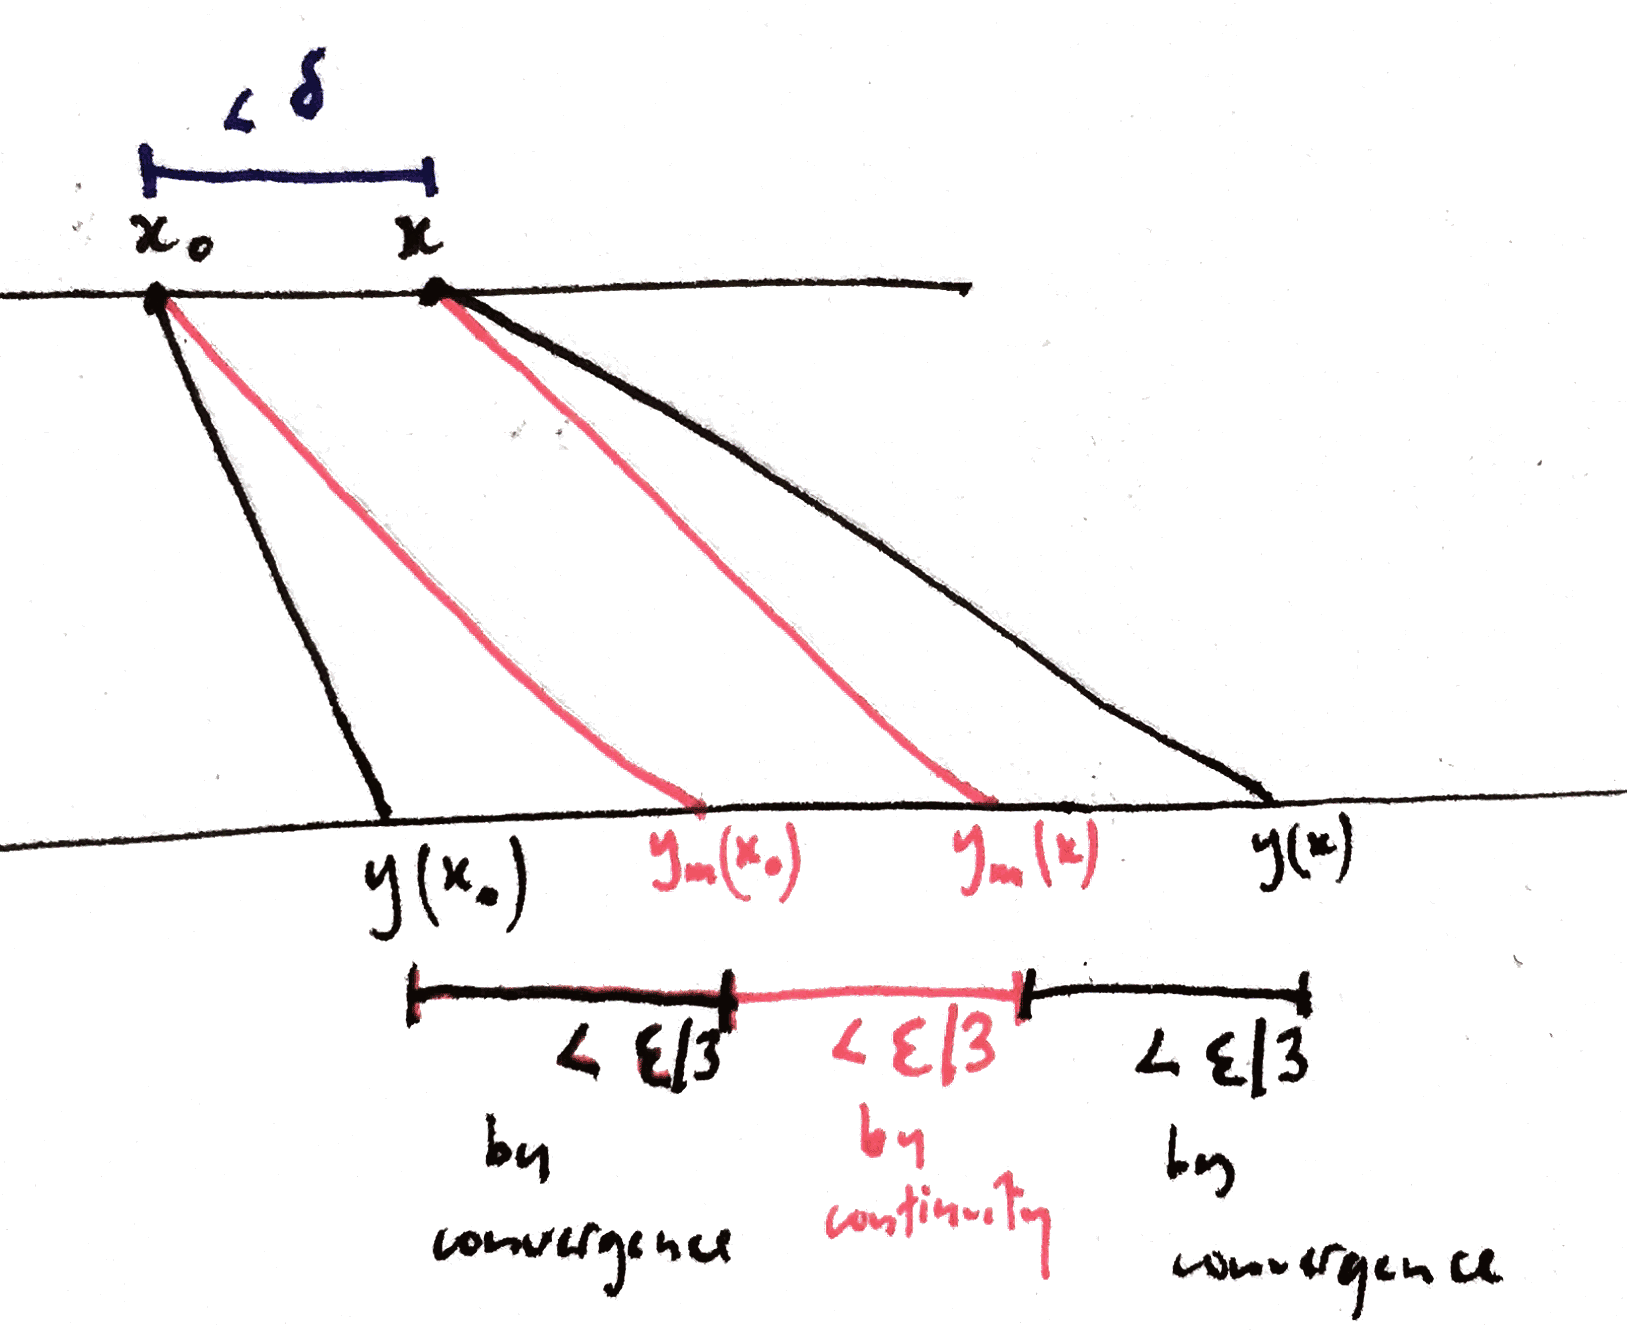
\includegraphics[width=200pt]{img/differential-equations-a1-1-1-a-diagram.png}\\

  % We need to show that for every $\epsilon > 0$, for every $x_0 \in [a, b]$,
  % there exists a $\delta > 0$ such that
  % $|x - x_0| < \delta \implies |y(x) - y(x_0)| < \epsilon$.

  Fix arbitrary $\epsilon > 0$ and $x_0 \in [a,b]$.

  Let $m \in \N$ be such that $|y_m(x_0) - y(x_0)| < \epsilon/3$. Such an $m$
  exists because the $\{y_n\}$ converge uniformly to $y$.

  Let $\delta$ be such that
  $|x - x_0| < \delta \implies |y_m(x) - y_m(x_0)| < \epsilon/3$. Such a
  $\delta$ exists because $y_m$ is continuous on $[a,b]$.

  Fix an arbitrary $x$ such that $|x - x_0| < \delta$.

  Now we have the following:
  \begin{enumerate}
  \item $|y(x_0) - y_m(x_0)| < \epsilon/3$ ~~~~ by convergence of the $\{y_n\}$
  \item $|y_m(x_0) - y_m(x)| < \epsilon/3$ ~~~ by continuity of $y_m$
  \item $|y_m(x) - y(x)| < \epsilon/3$    ~~~~~~ by convergence of the $\{y_n\}$
  \end{enumerate}
  Therefore $|y(x_0) - y(x)| < \epsilon$, proving continuity of $y$ on $[a,b]$. \qed

  \blue{(Approximate time taken for reading and producing an answer: 4hrs)}

  \subsubsection*{(c) Show limit of definite integral I}

  Let $I_n = \int_a^b |y_n(x) - y(x)| \dx$.

  The claim is that $\lim_{n \to \infty} I_n = 0$.

  In other words
  $\forall \epsilon > 0: \exists~ m \in \N: \forall~ n > m: |I_n - 0| <
  \epsilon$.

  Fix an $\epsilon > 0$.

  Since the $\{y_n\}$ converge uniformly to $y$, there exists an $m \in \N$
  such that for all $n > m$ and for all $x \in [a,b]$
  \begin{align*}
    |y_n(x) - y(x)| < \epsilon/(b-a).
  \end{align*}

  Therefore $\int_a^b |y_n(x) - y(x)| \dx < \epsilon$ for all $n > m$, as required. \qed

  \subsubsection*{(d) Show limit of definite integral II}

  The claim is that $\lim_{n \to \infty} \int_a^b y_n(x) \dx = \int_a^b y(x) \dx$.

  In other words:
  $\forall \epsilon > 0: \exists~ m \in \N: \forall~ n > m:$
  \begin{align*}
    \Big|\(\int_a^b y_n(x) \dx\) - \(\int_a^b y(x) \dx\)\Big| < \epsilon.
  \end{align*}

  This is equivalent to:
  $\forall \epsilon > 0: \exists~ m \in \N: \forall~ n > m:$
  \begin{align*}
    A_1 := \Big|\int_a^b \(y_n(x) - y(x)\) \dx\Big| < \epsilon.
  \end{align*}

  From part (c) above, we know that:
  $\forall \epsilon > 0: \exists~ m \in \N: \forall~ n > m:$
  \begin{align*}
    A_2 := \int_a^b |y_n(x) - y(x)| \dx < \epsilon.
  \end{align*}

  Now\footnote{How do I prove this section properly?} if the sign of $y_n(x) - y(x)$ is constant for all $x \in [a,b]$
  (i.e. the graphs do not cross over), then $A_1 = A_2 < \epsilon$. Otherwise,
  there is some cancellation in the integral $A_1$ and
  $0 \leq A_1 < A_2 < \epsilon$. So the same choice of $m$ as was used in part
  (c) works here, since for that value of $m$, we have $A_1 < \epsilon$ as
  required. \qed

  \blue{(Approximate time taken for (c) and (d): 2hrs)}
\end{mdframed}

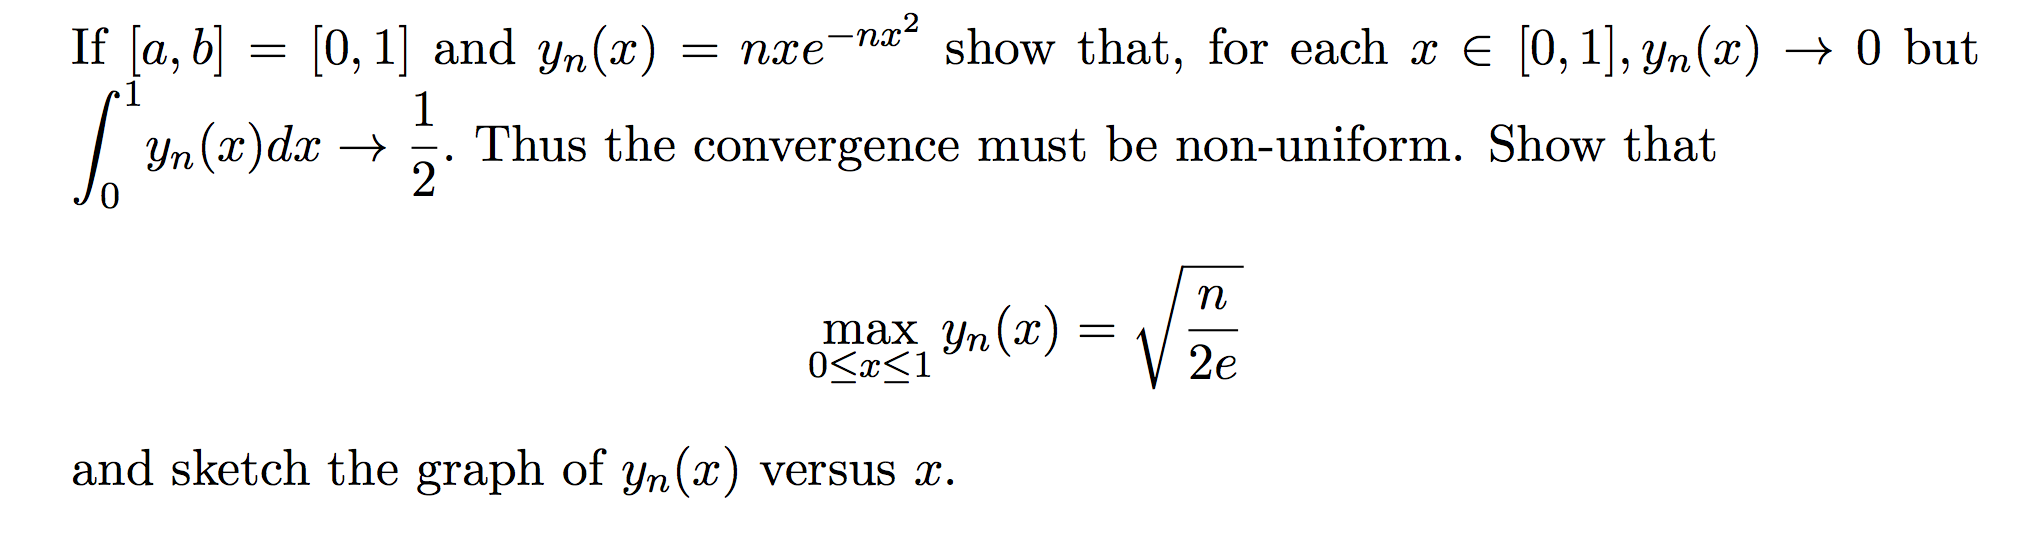
\includegraphics[width=450pt]{img/differential-equations-a1-1-1-b.png}\\
\begin{mdframed}
To show that $y_n(x) := \frac{nx}{e^{nx^2}} \to 0$ for all $x \in [0,1]$, first note that it is true
for $x = 0$ since $y_n(0) = 0$ for all $n \in \N$. So we have to show it is
true for $x \in (0, 1]$.

Fix $x \in (0, 1]$ and define $f(\alpha) = \frac{\alpha x}{e^{\alpha x²}}$
for $\alpha \in \R$.  $\lim_{\alpha \to \infty} f(\alpha)$ is an
indeterminate form $\frac{\infty}{\infty}$ and we can use l'H\^{o}pital's
rule, differentiating with respect to $\alpha$:
\begin{align*}
  \lim_{\alpha \to \infty} \frac{\alpha x}{e^{\alpha x^2}}
  = \lim_{\alpha \to \infty} \frac{x}{x^2e^{\alpha x^2}} = 0.
\end{align*}

Since $f(\alpha) = y_n$ at integer values of $\alpha$ it follows that
$\lim_{n\to\infty}y_n(x) = 0$ for all $x \in (0, 1]$. \qed

For the limit of the definite integral we have
\begin{align*}
  \int_0^1 nxe^{-nx^2} \dx
  = \Big[-\frac{1}{2}e^{-nx^2}\Big]_0^1 = \frac{1}{2}(1 - e^{-n}),
\end{align*}
and so $\lim_{n \to \infty} \int_0^1 y_n(x) \dx = \frac{1}{2}$. \qed

To find the maximum value attained by $y_n(x)$ for $x \in [0,1]$, note that the
derivative is
\begin{align*}
  \frac{\d y_n(x)}{\dx} = nx(-2nx)e^{-nx^2} + ne^{-nx^2} = ne^{-nx^2}(1 - 2nx^2),
\end{align*}
and therefore that the only solution to $\frac{\d y_n(x)}{\dx} = 0$ for
$x \in [0,1]$ is $x = \frac{1}{\sqrt{2n}}$.

The second derivative is
\begin{align*}
  % \frac{\d}{\dx} ne^{-nx^2}(1 - 2nx^2) =
  ne^{-nx^2}(-4nx) -2n^2xe^{-nx^2}(1 - 2nx^2)
  = 2n^2xe^{-nx^2}\(2nx^2 - 3\).
\end{align*}
This is negative at the critical point $x = \frac{1}{\sqrt{2n}}$ showing that
it is a maximum. Therefore
\begin{align*}
  \max_{x \in [0,1]} y_n(x)
  = n\frac{1}{\sqrt{2n}}e^{-n(\frac{1}{\sqrt{2n}})^2}
  = \sqrt{\frac{n}{2e}}. \qed
\end{align*}
\blue{(Approximate time for reading and producing answer: 3 hrs)}
\end{mdframed}

\end{document}
